\documentclass{article}
\usepackage[obeyspaces]{hyperref}
\usepackage[utf8]{inputenc}
\usepackage{graphicx}

\usepackage{float}
\usepackage[table,xcdraw]{xcolor}
\usepackage[tableposition=top]{caption}
\usepackage[T1]{fontenc}
\usepackage{kantlipsum}
\usepackage[usenames,dvipsnames]{xcolor}
\usepackage[breakable, theorems, skins]{tcolorbox}
\tcbset{enhanced}

\newcommand{\shellcmd}[1]{\\\indent\indent\texttt{\footnotesize\$ #1}\\}

\DeclareRobustCommand{\docBox}[2][gray!20]{%
\begin{tcolorbox}[   %% Adjust the following parameters at will.
        breakable,
        left=0pt,
        right=0pt,
        top=0pt,
        bottom=0pt,
        colback=#1,
        colframe=#1,
        width=\dimexpr\textwidth\relax, 
        enlarge left by=0mm,
        boxsep=5pt,
        arc=0pt,outer arc=0pt,
        ]
        #2
\end{tcolorbox}
}

\title{SimComp - Guide}
\author{Ole Bjørn Eithun Pedersen}
\date{June 2018}

\begin{document}

\maketitle
\tableofcontents
\newpage
\section{Introduction} \label{intro}
This document will serve as a quick start guide for the SimComp project. First, you should learn how to download (\ref{nedlasting}), update (\ref{oppdatere}) and build (\ref{bygge}) the project. As you will discover in these sections, all source code and binaries are available at \href{https://github.com/LasseNatvig/SimComp}{Github}. Already compiled versions (executable files) of the console and the graphical user interface can be found under \href{https://github.com/LasseNatvig/SimComp/releases/tag/v1.0}{realeases}. A short guide on how to use the applications is found in the \href{https://github.com/LasseNatvig/SimComp/wiki}{wiki}.  
\\
\\
To follow this guide using Windows you'll need Visual Studio 2017 or newer installed. If you're using Mac OS or Linux you'll need \href{https://git-scm.com/downloads}{Git} installed. Also, the guide presupposes that you already have a \href{https://www.github.com}{Github}-account.
\section{Download (Cloning)}
\label{nedlasting}
If you already have the project stored locally on you're machine, you can safely skip to (\ref{oppdatere}).
\subsection{Mac OS or Linux}
\begin{enumerate}
    \item Open a \textit{Terminal} window.
    \item Configuration of \textit{Git} (Skip if already configured):
        \begin{enumerate}
            \item Setting your username in \textit{Git} [\ref{username}]:
            \shellcmd{git config --global user.name "Mona Lisa"}
            \\The username is used by \textit{Git} to identify your commits. It doesn't have to be the same as on your \textit{Github}-account.
            \item Setting your commit email address in \textit{Git} [\ref{email}]:
            \shellcmd{git config --global user.email "email@example.com"}
            \\The email address should be the same as the one associated with your \textit{Github}-account.
        \end{enumerate}
    \item Enter the command:
    \\
    $$\shellcmd{git clone https://github.com/LasseNatvig/SimComp.git <PATH/NEWFOLDER>}$$
    \\
    PATH should be replaced with the path to where you want to store the project. NEWFOLDER should be replaced by the folder name in which to store the project.
    \item If the download was successful you should be able to change to that directory and list the content. Test by entering the following commands:\\
    $$\shellcmd{cd <PATH/NEWFOLDER>}$$
    $$\shellcmd{ls}$$\\
    The content should look something like this:\\
    $$\texttt{LICENSE  README.md   \_Console   \_GUI   \_Simulator   \_Wiki}$$\\
    
\end{enumerate}

\subsection{Windows}
\begin{enumerate}
    \item Open \textit{Visual Studio 2017}.
    \item Click on the \textit{View} button in the menu bar, then choose \textit{Team Explorer}.
    \item In the \textit{Team Explorer} window click \textit{Clone} under  \textit{Local Git Repositories}.
    \item In the top field, paste: \url{https://github.com/LasseNatvig/SimComp.git}. Then click on \textit{Clone}. The project will be saved in the folder given by the input field underneath.
\end{enumerate}
If the cloning was successful, you should have a folder named \textit{SimComp} under \textit{Local Git Repositories}.
\section{Update (Sync/Pull)} \label{oppdatere}

The version control system \textit{Git} uses branches, each branch contains a version of the project. The branch named \textit{Master} is often suppose to be a working version without bugs, it is most likely the branch you want to update. 
\subsection{Mac OS or Linux}
\begin{enumerate}
    \item Open a \textit{Terminal} window
    \item Change to the project directory:
    \shellcmd{cd <PROJECTPATH>}
    \item Update branches:
    \shellcmd{git fetch}
    \item  Make sure that you're on the right branch (Skip if you already know):
    \begin{enumerate}
        \item List branches:
        \shellcmd{git branch} \\
        The * symbol indicates the branch that you're on.  
        \item Change branch if necessary:
        \shellcmd{git checkout <BRANCH>}
    \end{enumerate}
    \item Update branch from remote (\textit{Github}):
    \shellcmd{git pull}
    \item Make sure that everything is up-to-date:
    \shellcmd{git status}\\
    This should display the message: \\
    "\texttt{On branch <BRANCH>\\
    Your branch is up-to-date with 'origin/<BRANCH>'.\\
    nothing to commit, working tree clean}"
    
\end{enumerate}

\subsection{Windows}
\begin{enumerate}
    \item Open \textit{Visual Sudio 2017}.
    \item Navigate to \textit{File} \(\rightarrow\) \textit{Folder} \(\rightarrow\) \textit{Open} in the menu bar.
    \item Choose the \textit{SimComp} folder.
    \item Navigate to \textit{View} \(\rightarrow\) \textit{Team Explorer} in the menu bar.
    \item In the \textit{Team Explorer}-window, click on \textit{SimComp} under \textit{Local Git Repositories}.
    \item Make sure that you're on the right branch (Skip if you already know):
        \begin{enumerate}
            \item Click on \textit{Branches} under \textit{project}.
            \item Under \textit{Active Git Repositories}, make sure that the name of the branch you wish to update is the one enclosed in parenthesis next to "SimComp".
            \item If you wish to change branch you'll have to double click that branch. \textbf{Note} that branches that does not exist locally is found under \textit{remotes/origin}.
            \item Navigate one page back by clicking the back button in the top left corner. 
        \end{enumerate}
    \item Click on \textit{Sync} under \textit{project}.
    \item Sync by clicking \textit{Sync}.
    \item A successful update(sync) is indicated by the message: \textit{Successfully synchronized incoming and outgoing commits.}
\end{enumerate}

By now the project should be up to date and ready to be built.\\
\textbf{Note} that if you're on a different branch than \textit{Master}, the code might not compile.
\newpage
\section{Build} \label{bygge}
The project has two user interfaces, one by console and one by graphics. Each of the two has its own directory with its own build configuration. Even though the code for the simulator is in a different directory, both user interfaces depend on it. The two user interfaces, on the other hand, is independent of each other. Therefore, the two UIs should also be built independently of each other. More information on the project structure is available on \href{https://github.com/LasseNatvig/SimComp}{Github}.
\\
\\
Follow the instructions in section (\ref{konsoll}) and (\ref{GUI}) to build the console- and GUI application respectively.

\subsection{Console} \label{konsoll}
The console application only depends on the C++11 standard library. Therefore it can be built as any other C++ project. However, the project provides some convenient files for doing so. If you're using Mac OS or Linux, we will show you how to build the project using \href{https://cmake.org}{\textit{CMake}} and \textit{Make}. On Windows, you can build the project using the provided \texttt{\textunderscore Console/\textunderscore src/SimComp\textunderscore Console.vcxproj} \textit{MSVS} project file.
% NOTE: Lasse: ... fant ingen filer i første omgang, men etterhvert, hvordan? ---- prøvde build på main.cpp, fungerte ikke ... sasm-filer må kopieres inn der exe filen ligger
%
\subsubsection{Mac OS or Linux}
\begin{enumerate}
    \item Open a \textit{Terminal} window
    \item Change to the project directory:
    \shellcmd{cd <PROJECTPATH>}
    \item Change to \texttt{\textunderscore Console/\textunderscore src/} folder:
    \shellcmd{cd \textunderscore Console/\textunderscore src/}
    \item Generate a \textit{makefile} with \textit{CMake}:
    \shellcmd{cmake .}
    \item Build using \textit{Make}:
    \shellcmd{make} \\
    This will build the project into an executable named "SimComp".
\end{enumerate}

\subsection{GUI} \label{GUI}
There are several ways to build this project. If you're using Windows, we will show you how to build it using \textit{Visual Studio}. On Mac OS or Linux we will show you how to build it using \textit{Qt Creator}. Either way you'll need \href{https://www.qt.io/download}{\textit{Qt}} versio 5.10 or newer. If you're building using \textit{Visual Studio} you'll also need \href{https://marketplace.visualstudio.com/items?itemName=TheQtCompany.QtVisualStudioTools-19123}{\textit{Qt Visual Studio Tools}}.

\subsubsection{Mac OS or Linux}
\begin{enumerate}
    \item Open \textit{Qt Creator}
    \item Navigate to \textit{File} \(\rightarrow\) \textit{Open File or Project} in the menu bar
    \item Navigate to \textit{Build} \(\rightarrow\) \textit{Build All}
    \item To start the application click the green start button in the bottom left corner
\end{enumerate}
\subsubsection{Windows}
\begin{enumerate}
    \item Open \textit{Visual Studio 2017}.
    \item Navigate to \textit{File} \(\rightarrow\) \textit{Open} \(\rightarrow\) \textit{Project/Solution}
    \item Choose \path{SimComp/_GUI/_src/SimComp_GUI.vcxproj}.
    % NOTE: ... add or close solution ? --- Lasse did close ?
    \textbf{Note} that there may appear a dialog window with information about \textit{Git}. It says that the changes in the console-project not will be tracked by \textit{Git}. Just press ok.
    \item Configuration of \textit{Qt Visual Studio Tools} (Skip if it is already configured):
        \begin{enumerate}
        % NOTE: Lasse did not need to do this, had Qt already installed? Try again on a new "empty" computer
            \item Navigate to \textit{Qt VS Tools} \(\rightarrow\) \textit{Qt Options} in the menu bar. 
            \item Click \textit{Add} in the popup window. 
            \item In the window \textit{Add new Qt version} you'll have to choose the \textit{Qt}-version that you'd like to use. Paste the path or click [...] to choose the folder \path{msvc2017_64} under \path{Qt/<VERSION>/}.
        \end{enumerate}
    \item You can now build the project like any other \textit{Visual Studio}-project.
\end{enumerate}
\section{Simulator API Documentation}
The \texttt{ComputerSimulation} class defined in \texttt{\_Simulator/\_src/compSim.h} is the access point to the API. Therefore, all functions described below are member functions of the \texttt{ComputerSimulation} class.
\\ \\
\docBox {\texttt{typedef uint16\_t word}
\\ \small{Definition of word size.}
\\ \\
\texttt{ComputerSimulation(std::string name, std::string loggerFilename)}\\
\small{ Constructs an instance of the class with the given name (not important) and starts logging to the loggerFilename. \textbf{Note} that the simulator will overwrite existing files with the same filename as loggerFilename.}
\\ \\
\texttt{ComputerSimulation(std::string name)}
\\ \small{Same as above but will log to the standard \texttt{logg.txt} filename. }
\\ \\
\texttt{void load(std::string filename)}
\\ \small{Loads and parses sasm-file named \texttt{filename} to the simulator.}
\\ \\
\texttt{void reset()}
\\ \small{Sets the program counter and instruction count to zero, clears breakpoints, wipes instruction- and data memory and resets statistics.}
\\ \\
\texttt{void run()} 
\\ \small{Starts simulation from the program counter value to the last instruction (or next HLT instruction).}
\\ \\
\texttt{bool step()} 
\\ \small{Executes one step (instruction). Returns \texttt{true} if instruction is not HLT.}
\\ \\
\texttt{bool next()} 
\\ \small{Starts simulation. Stops at next breakpoint or HLT instruction. Returns \texttt{true} if last instruction is not HLT.} 
\\ \\
\texttt{void writeToLog(std::string message)}
\\ \small{Write \texttt{message} to log.}
\\ \\
\texttt{void resetStatistics()}
\\ \small{Reset simulator statistics.}
\\ \\
\texttt{std::vector<std::string> memoryDump(word fromAddr, word toAddr, memType memoryType)} 
\\ \small{If \texttt{memoryType == DATA} the returned vector is populated with hexadecimal values from data memory (one word per vector item). If \texttt{memoryType == INSTR} the returned vector is populated with disassembled instructions. The fromAddr and toAddr variables denotes the start and end address of the memory area that is dumped.}  
\\ \\
\texttt{word getPC() const}
\\ \small{Returns the program counter value.}
\\ \\
\texttt{long long getInstructionsSimulated() const}
\\ \small{Returns the number of instructions that has been simulated.}
\\ \\
\texttt{bool isRunning() const}
\\ \small{Returns \texttt{true} if the simulator is in RUN-mode.}
\\ \\
\texttt{bool singleStep() const}
\\ \small{Returns \texttt{true} if the simulator is in SINGLESTEP-mode.}
\\ \\
\texttt{bool validProgram() const}
\\ \small{Returns \texttt{true} if a valid program is loaded to the simulator.}
\\ \\
\texttt{word getInstr(word PC)}
\\ \small{Returns the instruction at the address pointed at by PC (program counter).}
\\ \\
\texttt{Mode getMode() const}
\\ \small{Returns the mode that the simulator is currently in.}
\\ \\
\texttt{std::string getName() const}
\\ \small{Returns simulator name as \texttt{std::string}.}
\\ \\
\texttt{void setBreakpoints(const std::vector<int> &breakpoints)}
\\ \small{Sets breakpoints at the line numbers(in the program file) given by the \texttt{breakpoints} vector.}
\\ \\
\texttt{void setPC(word PC)}
\\ \small{Sets program counter to \texttt{PC}.}
}
\section{Source Code Overview}
This section is intended to help you familiarize with the SimComp codebase. Since both UIs are dependent on the Simulator API it is crucial that you're familiar with it before you start this section. Figure \ref{fig:relation} shows the relation between the different parts of the SimComp project.

\begin{figure}[H]
\centering
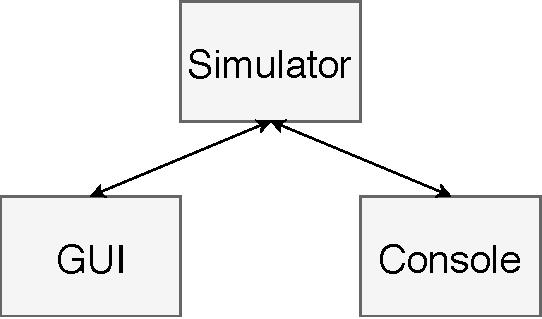
\includegraphics[scale=0.8]{img/SimComp-relation.pdf}
\caption{SimComp project relation}
\label{fig:relation}
\end{figure}

\subsection{Simulator}
\subsubsection{File Description}
\begin{description}
\item[isa.h/.cpp] - Contains the \texttt{Isa} class that defines the instruction set and functions that help interpreting and printing instructions.

\item[loader.h/.cpp] - Contains the \texttt{Loader} class that reads the sasm-format and generates instructions that are written to the instructions memory.

\item[logger.h/.cpp] - Contains the \texttt{Logger} class used to log simulator execution. 

\item[memory.h/.cpp] - Contains the \texttt{Memory} class used by the \texttt{ComputerSimulation} class to store data- and instruction memory. 

\item[program.h/.cpp] - Contains the \texttt{Program} struct that stores information about a assembler program, the struct is needed by \texttt{ComuputerSimulation} to generate instructions.

\item[compSim.h/.cpp] - Contains the \texttt{ComputerSimulation} class that is responsible for control and execution of simulation. The class is designed to be the access point for the API. 
\end{description}

\subsection{Console}
\subsubsection{File Description}
\begin{description}
\item[main.cpp] - Entry point that uses the first argument as the path to construct an instance of \texttt{ConsoleUi}. 

\item[consoleUI.h/.cpp] - Contains the class \texttt{ConsoleUi} which creates and controls a console user interface. \texttt{ConsoleUi} is also responsible for creating an instance of \texttt{ComputerSimulation}.
\item[config.h/.cpp] - Contains functions for finding assembler programs in a folder.
\item[utils.h/.cpp] - Contains utility functions for creating a console ui.
\end{description}

\subsection{GUI}
\subsubsection{File Description}
\begin{description}
\item[main.cpp] - Entry point. Starts application and creates an instance of \texttt{MainWindow}. 

\item [mainwindow.h/.cpp] - The \texttt{MainWindow} class inherits \texttt{QMainWindow}. It is responsible for creating and controlling all dock windows, the menubar, statusbar, styling and the central widget. The central widget is a \texttt{QTabWidget} populated with one instance of \texttt{RunWidget} and one of \texttt{IdeWidget}. Figure \ref{fig:qmainwindowlayout} shows how these are organized. For more information on \texttt{QMainWindow} see [\ref{qmainwindow}].

\begin{figure}[H]
\centering
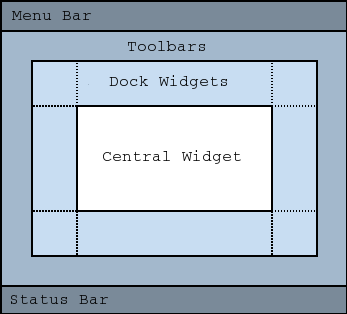
\includegraphics[scale=0.5]{img/mainwindowlayout.png}
\caption{QMainWindow layout \cite{qt}}
\label{fig:qmainwindowlayout}
\end{figure}


\item [runwidget.h/.cpp] - Contains the \texttt{RunWidget} and the \texttt{SimulatorThread} classes. \\ \\ \texttt{RunWidget} inherits \texttt{QWidget} and is responsible for simulator execution. Graphically, the widget consists of the execution table which show information relevant to execution, see figure \ref{fig:runwidget}. \texttt{RunWidget} is one of the two tabs in the \texttt{QTabWidget} set as central widget by \texttt{MainWindow}. \\ \\
\texttt{SimulatorThread} inherits \texttt{QThread}. The class overrides the \texttt{virtual void QThread::run()} function to start the simulator by invoking \texttt{void ComputerSimulation::run()}. Calling \texttt{SimulatorThread::run()} will therefore start the simulator in RUN-mode in a thread. The class is constructed with a pointer to a \texttt{ComputerSimulation} instance.

\begin{figure}[H]
\centering
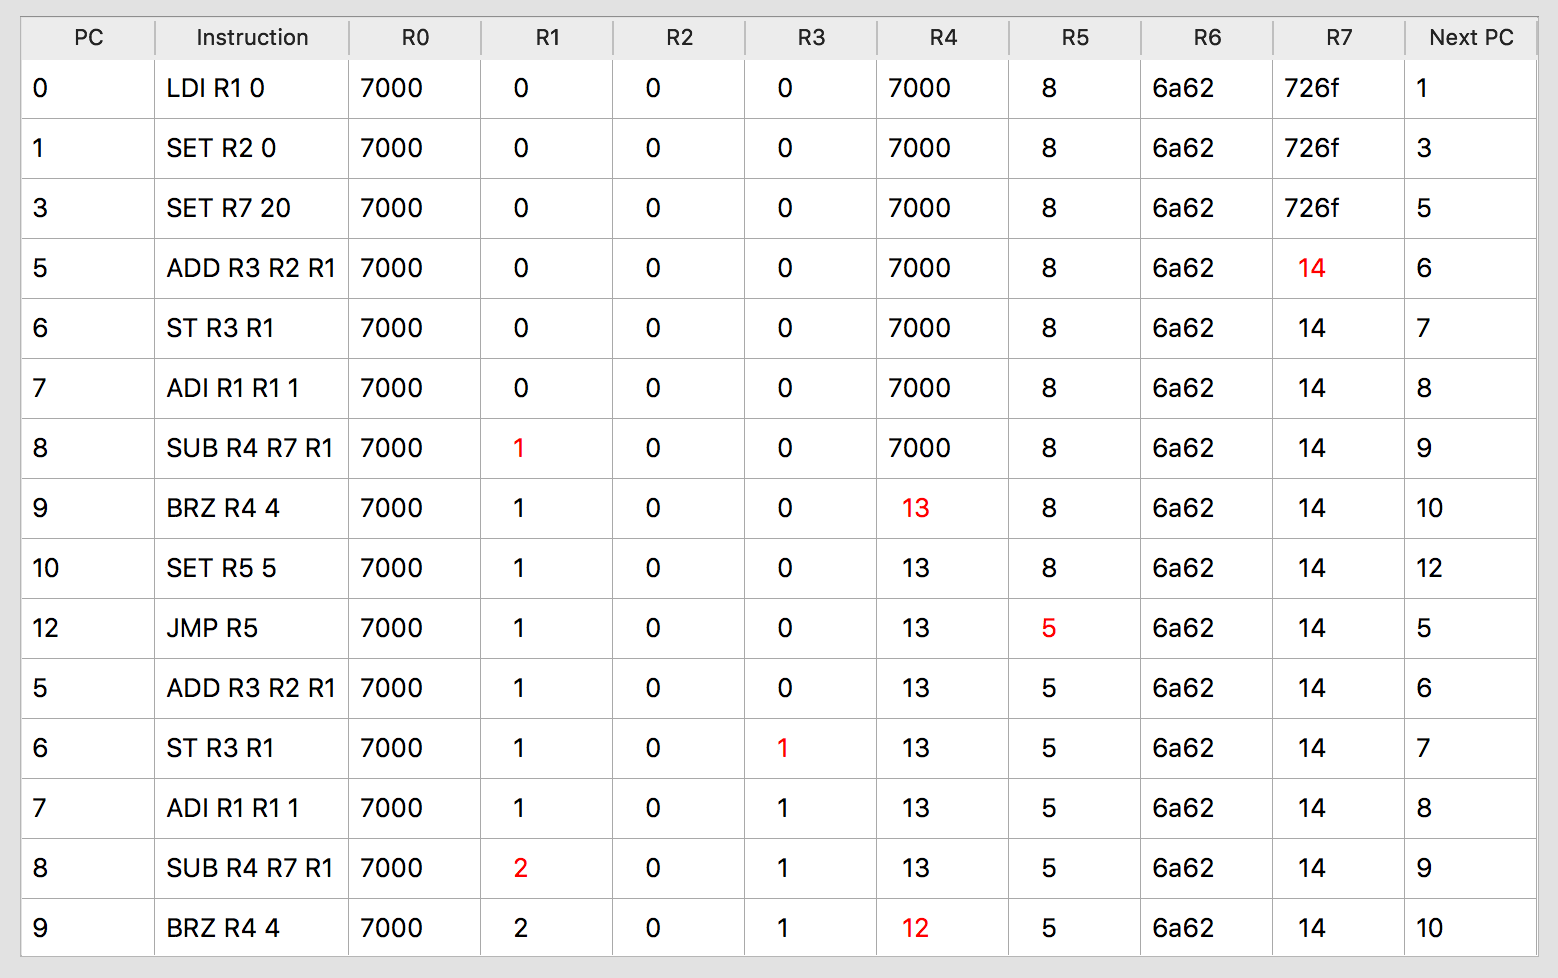
\includegraphics[scale=0.3]{img/RunWidget.png}
\caption{Screenshot of a RunWidget used in the SimComp GUI.}
\label{fig:runwidget}
\end{figure}


\item [idewidget.h/.cpp] - The \texttt{IdeWidget} class inherits \texttt{QPlainTextEdit} and acts as a standalone ide widget. Graphically, the widgets consists of the editing area and a left sidebar with line numbers and breakpoints, see figure \ref{fig:idewidget}. The class is responsible for creating, editing, opening and saving assembler programs. \texttt{IdeWidget} is the second of the two tabs in the \texttt{QTabWidget} set as central widget by \texttt{MainWindow}.

\begin{figure}[H]
\centering
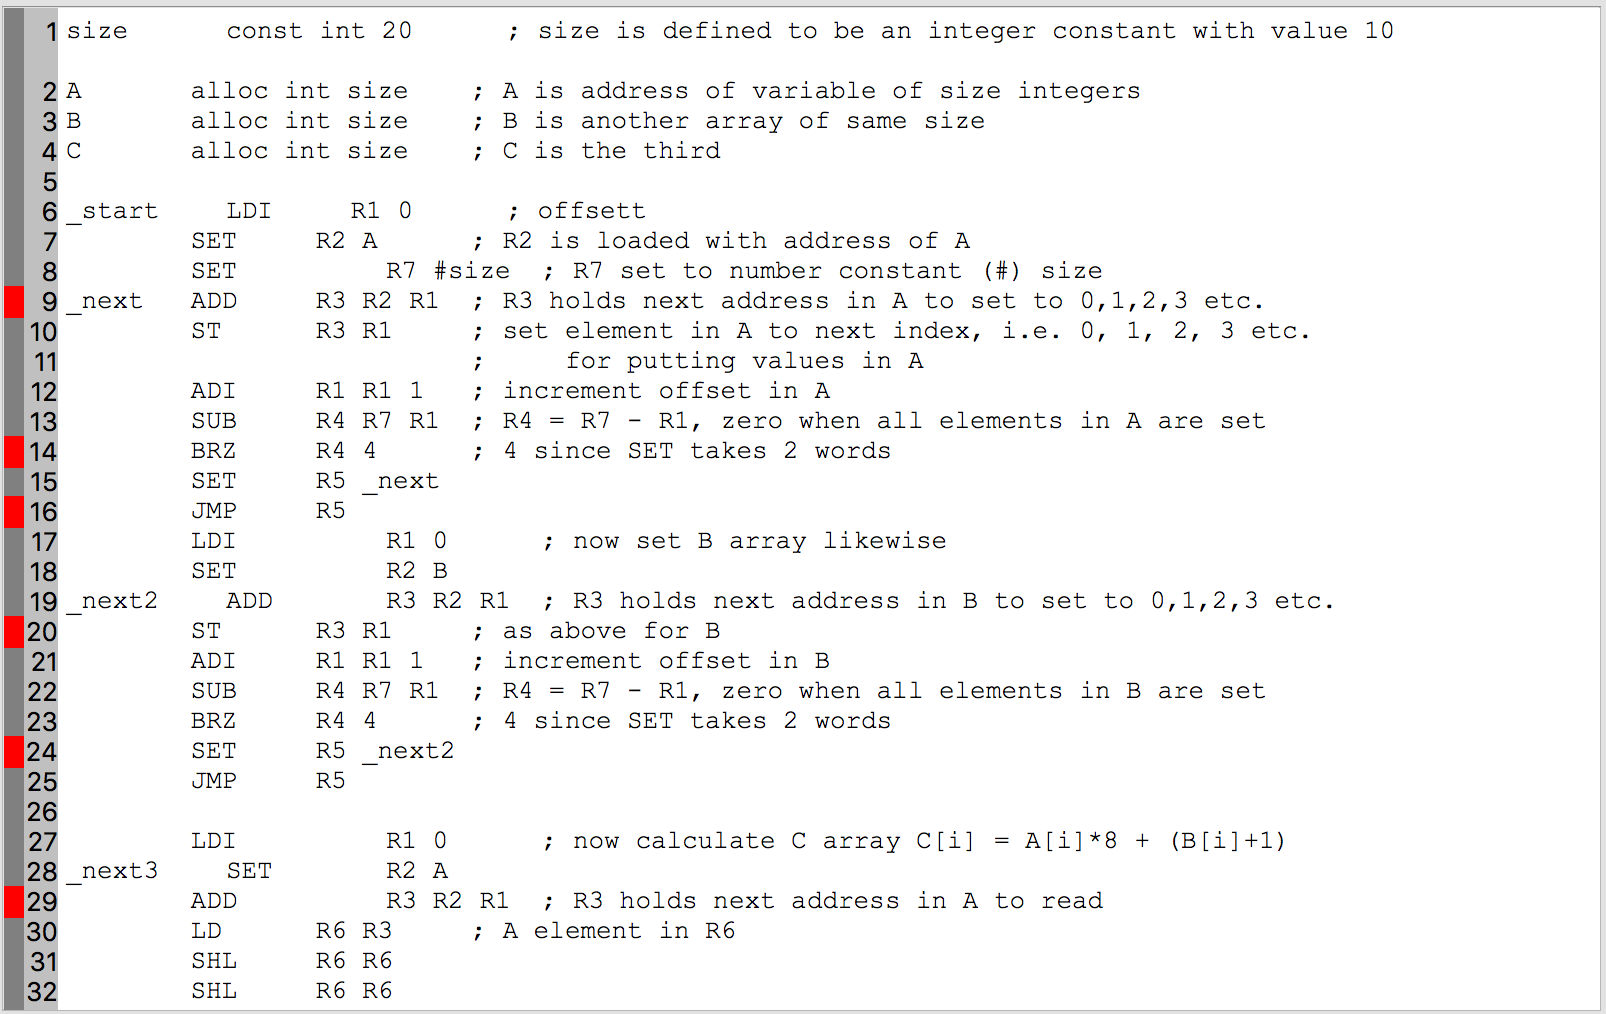
\includegraphics[scale=0.3]{img/IdeWidget.png}
\caption{Screenshot a IdeWidget used in the SimComp GUI.}
\label{fig:idewidget}
\end{figure}

\item [memorywindow.h/.cpp] - The \texttt{MemoryWindow} class inherits \texttt{QWidget} and is should be used as a top-level window. The window is used to display memory areas, see fig \ref{fig:memorywindow}. A \texttt{QSplitter} is used to fill the top layout of the window. The splitter is populated by two widgets: 

\begin{itemize}
    \item The left side is a \texttt{QTabWidget} that contains two tabs, one with a table- (\texttt{QTableWidget}) and one with an graphical (\texttt{MemoryMap}) representation of the memory area.
    \item The rigth side is a \texttt{QWidget} which is used as a container for the configuration portion of the \texttt{MemoryWindow}.
\end{itemize}

\begin{figure}[H]
\centering
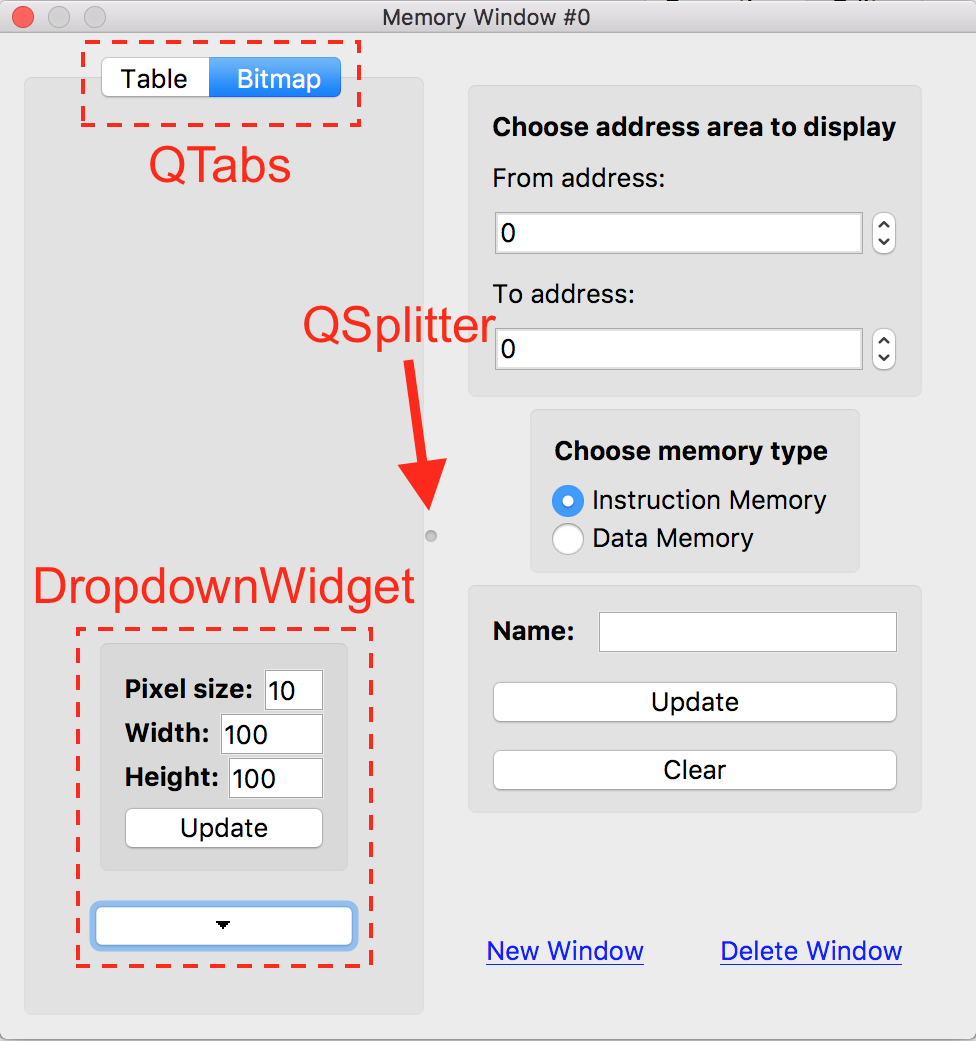
\includegraphics[scale=0.35]{img/MemoryWindow.png}
\caption{Screenshot of a MemoryWindow used in SimComp GUI.}
\label{fig:memorywindow}
\end{figure}

\item [memorymap.h/.cpp] - The \texttt{MemoryMap} class inherits \texttt{QWidget} and overrides the \texttt{virtual void QWidget::paintEvent(QPaintEvent *event)} function to paint it self as a bitmap with the values set in the member variable \texttt{hexMap}. The \texttt{hexMap} is a \texttt{std::vector<std::string>} and is set using the \texttt{setVector} member function.

\item [dropdownwidget.h/.cpp] - The \texttt{DropDownWidget} class inherits \texttt{QWidget}. It acts as a drop-down menu that can be populated with widgets using the \texttt{addWidget} function.

\item [fileviewer.h/.cpp] - The \texttt{FileViewer} class inherits \texttt{QWidget} and is responsible for displaying file information, see figure \ref{fig:fileviewer}. It also provides an additional way to choose assembler program. 

\begin{figure}[H]
\centering
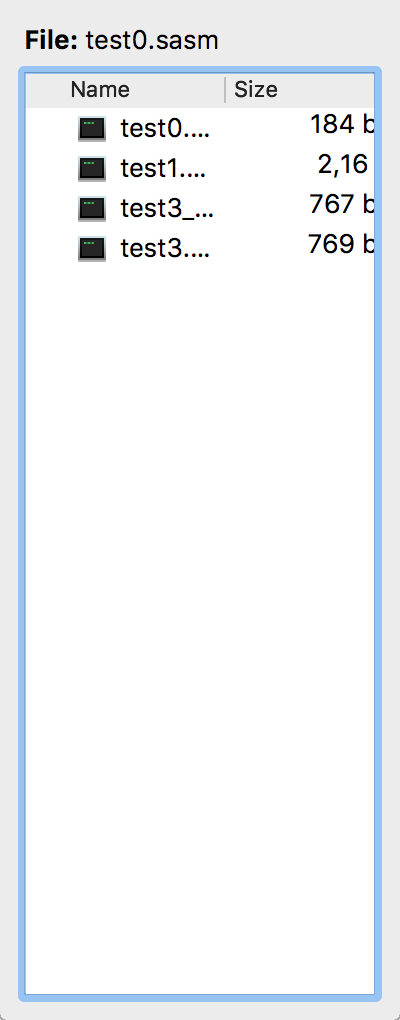
\includegraphics[scale=0.3]{img/FileViewer.png}
\caption{Screenshot of a FileViewer used in the SimComp GUI.}
\label{fig:fileviewer}
\end{figure}

\item [performancechart.h/.cpp] - The \texttt{PerformanceChart} inherits \texttt{QChart} and is used to display a live plot of the simulator performance (MIPS), see figure \ref{fig:performancechart}.

\begin{figure}[H]
\centering
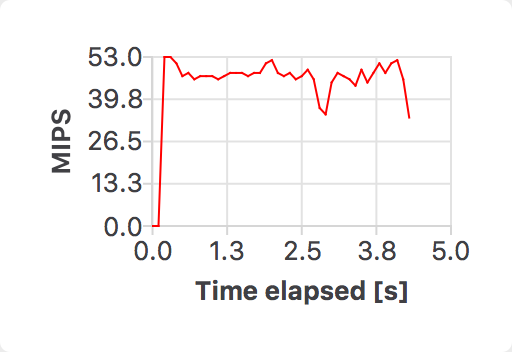
\includegraphics[scale=0.6]{img/PerformanceChart.png}
\caption{Screenshot of a PerformanceChart used in the SimComp GUI.}
\label{fig:performancechart}
\end{figure}

\item [globals.h] - Used to store global constants in the \texttt{globals} namespace.

\end{description}

\subsubsection{Important connections}
Qt Object Communication relies on sending and receiving signals. The receiver responds to a signal by calling a function (slot). The most important of these signal-slot connections are listed in table \ref{table:connections}. \textbf{Note} that Lambda* denotes C++11 lambda functions that are not members, therefore there is no receiver.
\begin{table}[H]
\caption{Important Qt connections in the SimComp GUI project.}
\makebox[\linewidth]{
\begin{tabular}{|l|l|l|l|}
\hline
\rowcolor[HTML]{C0C0C0} 
\textbf{Sender} & \textbf{Signal}                                     & \textbf{Receiver} & \textbf{Slot/Function}                                                                       \\ \hline
RunWidget       & instructionCountChanged(int) & Lambda*           & \begin{tabular}[c]{@{}l@{}}Updates status bar with\\ the new instruction count.\end{tabular} \\ \hline
RunWidget       & performanceChanged(double)               & PerformanceChart  & updatePerformance(double)                                                               \\ \hline
IdeWidget       & fileChanged(QString)                 & RunWidget         & load(QString)                                                                       \\ \hline
IdeWidget       & fileChanged(QString)                 & Lambda*           & Set FileViewer to filename.                                                                  \\ \hline
IdeWidget       & breakPointsChanged()                                & Lambda*           & \begin{tabular}[c]{@{}l@{}}Sets breakpoints in \\ RunWidget.\end{tabular}                    \\ \hline
FileViewer      & changeFile(QString)                  & IdeWidget         & open(QString)                                                                       \\ \hline
SimulatorThread & finished()                                          & RunWidget         & runFinished()                                                                                \\ \hline
QTimer          & timeout()                                           & RunWidget         & updatePerformance()                                                                          \\ \hline
\end{tabular}
}
\label{table:connections}
\end{table}

\section{Contributing}
Everyone is welcomed to contribute, but since this is a project made for students taking the \href{https://www.ntnu.edu/studies/courses/TDT4102}{TDT4102} NTNU course, their pull requests and issues will be prioritized. A detailed description on how to contribute will follow below.

\begin{enumerate}
    \item First, you'll need to fork the \href{https://github.com/LasseNatvig/SimComp}{\textit{Github}} repository by click on the "Fork"-button.
    \begin{figure}[H]
        \centering
        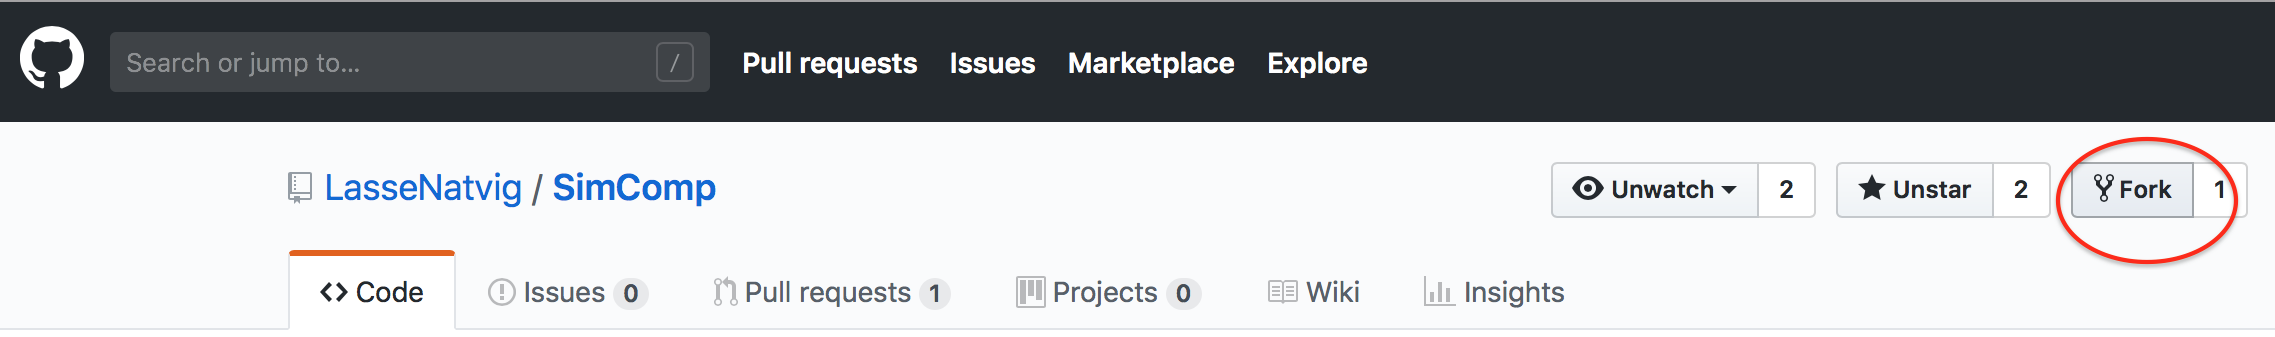
\includegraphics[scale=0.3]{img/Fork.png}
        \label{fig:fork}
    \end{figure}
    This will create version of the project on your \textit{Github}-account. 
    \item Next, follow section \ref{nedlasting} but replace the url in step 4 (3 on Linux/mac) with your own \texttt{https://github.com/<YOURUSERNAME>/SimCom.git} to download the project.
    \item Make changes to your version. Remember to push the changes to the remote (Github).
    \item Create a new pull request by click the "New pull request"-button in your fork. 
    \begin{figure}[H]
        \centering
        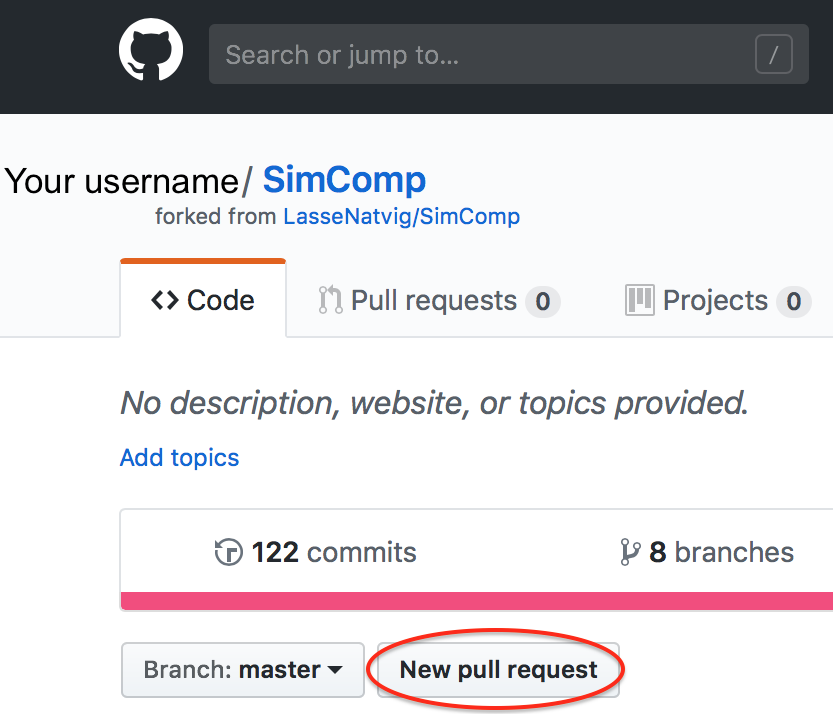
\includegraphics[scale=0.3]{img/Newpullrequest.png}
        \label{fig:fork}
    \end{figure}
    \item 
\end{enumerate}


\section{Troubleshooting}
Add potential problems with fixes!

\begin{thebibliography}{9}
\bibitem{setusername}\label{username}
  Setting your username in Git, \url{https://help.github.com/articles/setting-your-username-in-git/}, \date{23.06.2018}
\bibitem{setemail}\label{email}
    Setting your commit email address in Git, \url{https://help.github.com/articles/setting-your-commit-email-address-in-git/}, \date{23.06.2018}
\bibitem{qmainwindow}\label{qmainwindow}
    QMainWindow Class | Qt 4.8
    \url{http://doc.qt.io/archives/qt-4.8/qmainwindow.html}
    \date{05.07.2018}
\end{thebibliography}

\end{document}
%\begin{figure}[htbp]
 %   \centering
  %  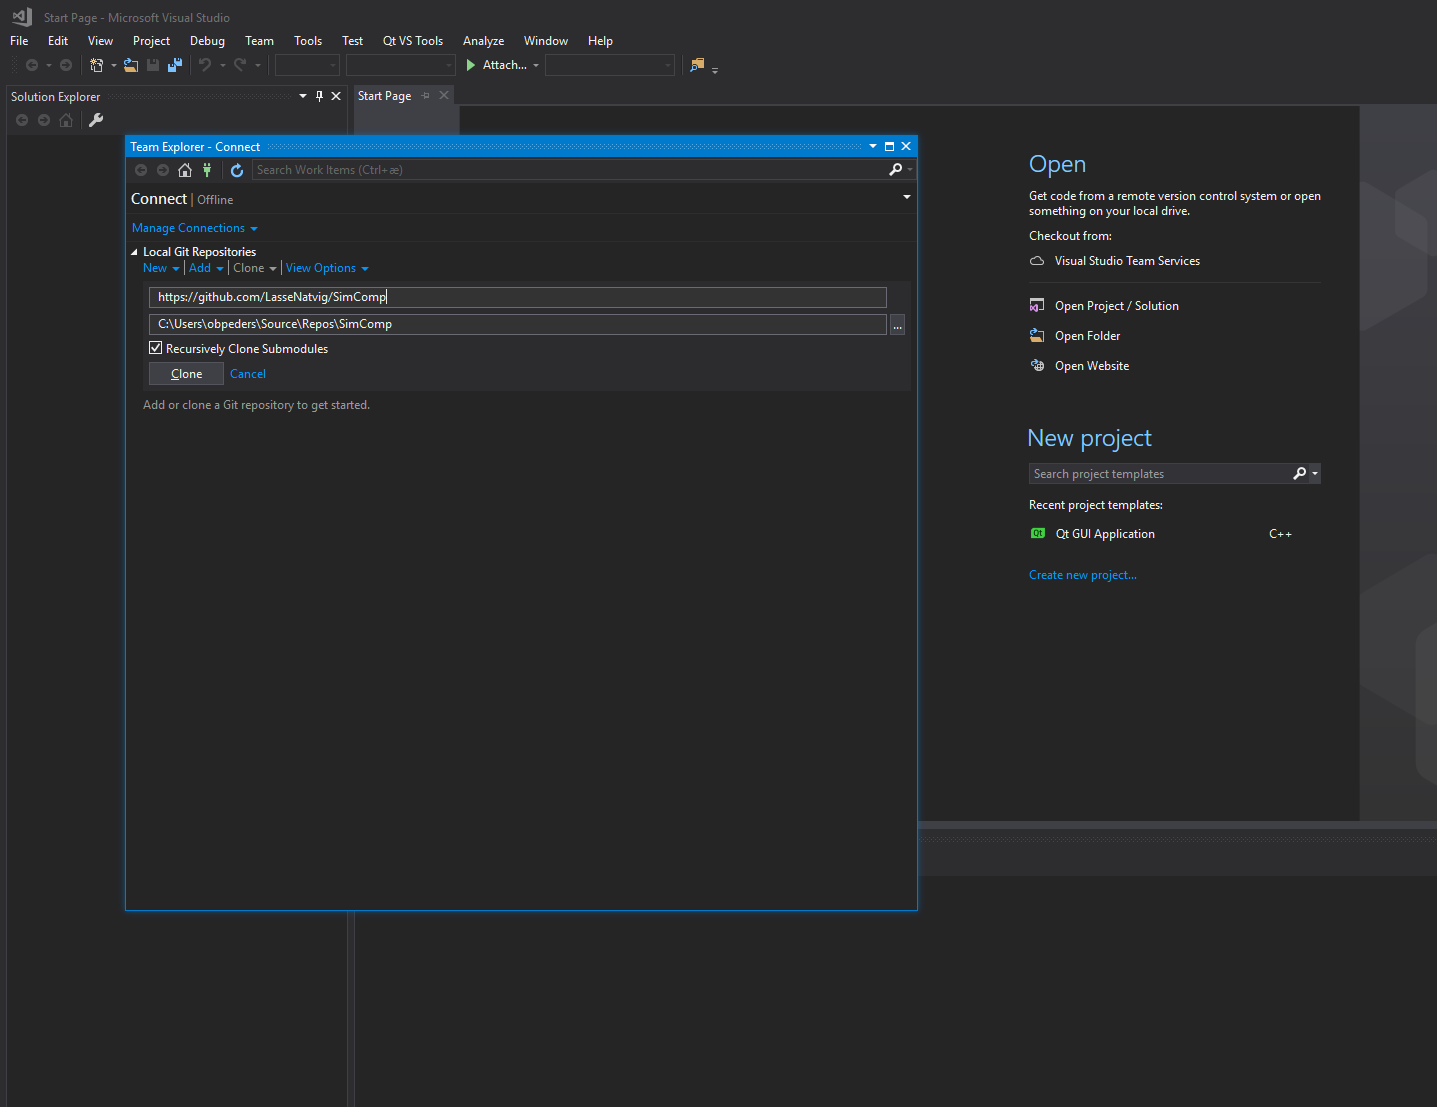
\includegraphics[scale=0.3]{img/fig1.PNG}
   % \label{fig:clone}
%\end{figure}